%%%%%%%%%%%%%%%%%%%%%%%%%%%%%%%%%%%%%%%%
% basic elements

\documentclass[12pt]{article}
\usepackage[english]{babel}
\usepackage{amsmath,amsthm}
\usepackage{amsfonts}
\usepackage{makecell}
\usepackage{graphics}
\usepackage{graphicx}
\usepackage{fancyhdr}
\usepackage{ifthen}
\usepackage{wrapfig}
\usepackage{array}
\usepackage{colortbl}
\usepackage{fullpage}
\usepackage[table]{xcolor}
\usepackage{subfigure}
\usepackage{caption}
\usepackage{float}
\usepackage{ctex}
\usepackage{appendix}
\usepackage{shorttoc}
\usepackage{pagenote}
\usepackage{setspace}
\usepackage{geometry}
\usepackage{indentfirst}
\usepackage{fullpage}
\usepackage{booktabs}
\usepackage{multirow}
\usepackage{longtable}
\usepackage{minipage-marginpar}
\usepackage{hyperref}
\usepackage{palatino}
\usepackage{setspace}
\usepackage{subfigure}
\usepackage{picinpar}
\usepackage{newtxtext}
\usepackage{amsmath,amssymb,amsthm}
\usepackage{newtxmath} % must come after amsXXX

% Replace ABCDEF in the next line with your chosen problem
% and replace 111111 with your Team Control Number
% and replace abcdef with your Title
% and replace 123456 with the number of pages of your essay
\newcommand{\Problem}{PROBLEM HERE}
\newcommand{\Team}{{TEAM HERE}}
\newcommand{\Title}{{TITLE HERE}}
\newcommand{\wholepages}{PAGE HERE}
\title{\huge\textbf{TITLE HERE}}
\author{Team\#\Team}
\date{\today}

%%%%%%%%%%%%%%%%%%%%%%%%%%%%%%%%%%%%%%%%
% set up of theorems

\newtheorem{thm}{Theorem}[section]
\newtheorem{cor}[thm]{Corollary}
\newtheorem{lem}[thm]{Lemma}
\newtheorem{prop}[thm]{Proposition}
\theoremstyle{definition}
\newtheorem{defn}[thm]{Definition}
\theoremstyle{remark}
\newtheorem{rem}[thm]{Remark}
\numberwithin{equation}{section}
\newtheorem{theorem}{Theorem}
\newtheorem{corollary}[theorem]{Corollary}
\newtheorem{lemma}[theorem]{Lemma}
\newtheorem{definition}{Definition}

%%%%%%%%%%%%%%%%%%%%%%%%%%%%%%%%%%%%%%%%
% setup of page length and script size

\setlength{\belowcaptionskip}{9pt}
\setlength{\abovecaptionskip}{9pt}
\setlength{\headsep}{0.4in}
\setlength{\headheight}{14.5pt}
\captionsetup{font={footnotesize}}
\renewcommand{\baselinestretch}{1.1}
\geometry{bottom=1in}

%%%%%%%%%%%%%%%%%%%%%%%%%%%%%%%%%%%%%%%%
% set up of page style

\pagestyle{fancy}
\fancyhead[L]{Team\ \#\Team}
\fancyhead[C]{\Title}
\fancyhead[R]{Page \thepage \ of \wholepages}
\fancyfoot{}

%%%%%%%%%%%%%%%%%%%%%%%%%%%%%%%%%%%%%%%%
% hyphenation

\tolerance=1
\emergencystretch=\maxdimen
\hyphenpenalty=10000
\hbadness=10000

\hypersetup{hidelinks} 
\hypersetup{
	colorlinks=false,
	linkcolor=black,
	citecolor=black,
	anchorcolor=black
}

%%%%%%%%%%%%%%%%%%%%%%%%%%%%%%%%%%%%%%%%
% biblography
\bibliographystyle{plain}
% \usepackage{url}
% \def\UrlBreaks{\do\A\do\B\do\C\do\D\do\E\do\F\do\G\do\H\do\I\do\J\do\K\do\L\do\M\do\N\do\O\do\P\do\Q\do\R\do\S\do\T\do\U\do\V\do\W\do\X\do\Y\do\Z\do\[\do\\\do\]\do\^\do\_\do\`\do\a\do\b\do\c\do\d\do\e\do\f\do\g\do\h\do\i\do\j\do\k\do\l\do\m\do\n\do\o\do\p\do\q\do\r\do\s\do\t\do\u\do\v\do\w\do\x\do\y\do\z\do\.\do\@\do\\\do\/\do\!\do\_\do\|\do\;\do\>\do\]\do\)\do\,\do\?\do\'\do+\do\=\do\#}

%%%%%%%%%%%%%%%%%%%%%%%%%%%%%%%%%%%%%%%%
% end of the beginning part
\begin{document}
	\DeclareGraphicsExtensions{.pdf, .jpg, .tif, .png}
	\thispagestyle{empty}
	\vspace*{-16ex}
	% MCM/ICM Template
	% \centerline{\begin{tabular}{*3{c}}
			%	\parbox[t]{0.3\linewidth}{\begin{center}\textbf{Problem Chosen}\\ \Large \Problem\end{center}}
			%	& \parbox[t]{0.3\linewidth}{\begin{center}\textbf{2020\\ MCM \\ Summary Sheet}\end{center}}
			%	& \parbox[t]{0.3\linewidth}{\begin{center}\textbf{Team Control Number}\\ \Large Team \# \Team\end{center}}	\\
			%	\hline
			%\end{tabular}}

	% HiMCM/IMMC Template
	\begin{center}
		\centerline{\begin{tabular}{p{\linewidth}<{\centering}}
				\small Team Control Number \\
				\huge \textbf{\Team} \\
				\small Problem Chosen \\
				\huge \textbf{\Problem} \\
				\textbf{2022} \\
				\small \textbf{IMMC Greater China Region} \\
				\small \textbf{Summary Sheet} \\
				\hline
		\end{tabular}}
	\end{center}
%%%%%%%%%%% Begin Summary %%%%%%%%%%%%%%%%%%
% Enter your summary here replacing the (red) text
% Replace the text from here ...
\qquad
\par

SUMMARY HERE

% to here
%%%%%%%%%%% End Summary %%%%%%%%%%%%%%%%%%%
\thispagestyle{empty}
\maketitle
\thispagestyle{empty}
\newpage
%%%%%%%%%%%%%%%%%%%%%%%%%%%%%%%%%%%%%%%%
\clearpage
\thispagestyle{empty}
% Uncomment the next line to generate a Table of Contentsr%r%\shortableofcontents{Contents}{2}
\tableofcontents % Uncomment this line to update the Contents
\newpage
\pagestyle{fancy}
\setcounter{page}{1}
% Begin your paper here
%%%%%%%%%%%%%%%%%%%%%%%%%%%%%%%%%%%%%%%%

\newpage
\section{Introduction}

	\subsection{Background}
		BACKGROUND \cite{LIKE THIS}


		\begin{center}
		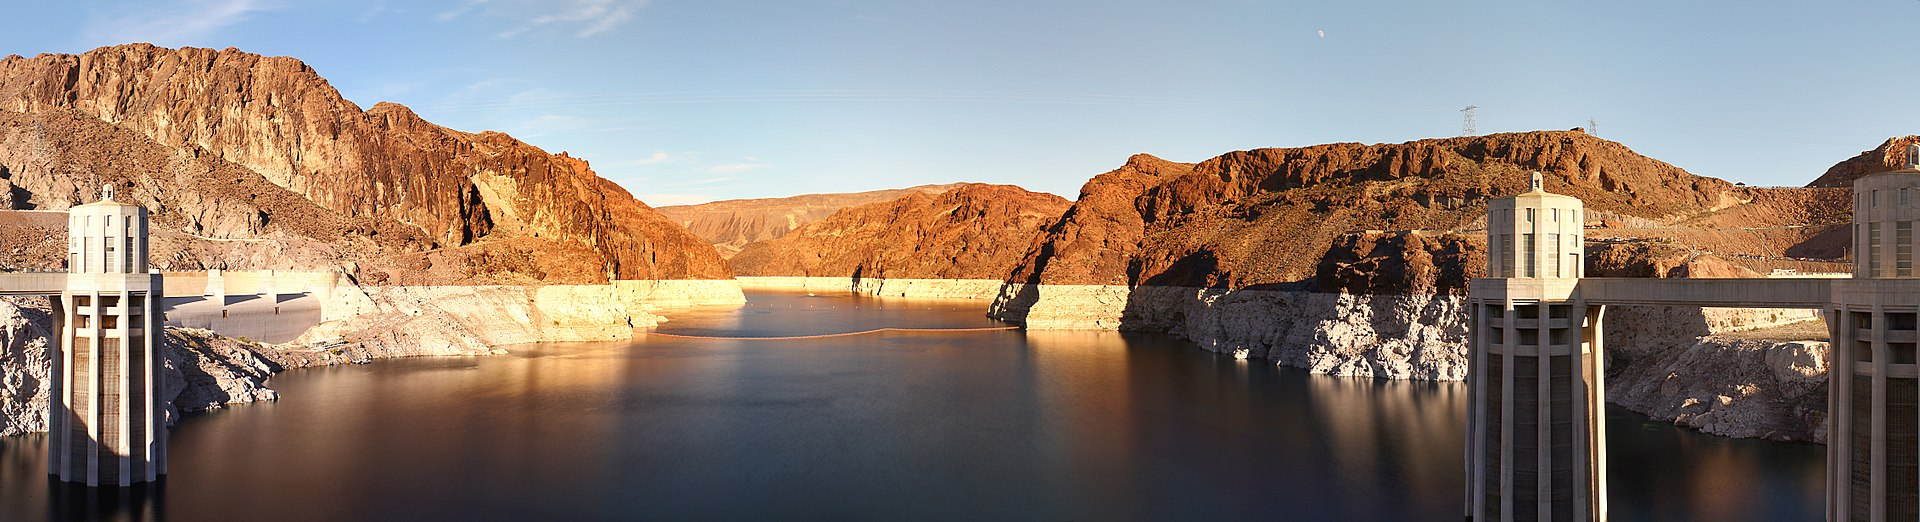
\includegraphics[width=13cm]{1.1 GRAPHICS.jpg}

		\small \textit{Fig. 1.1 GRAPHICS}
		\end{center}

	\subsection{Problem Restatement}

	\subsection{General Assumptions}

\newpage
\section{Overall Analysis}

	\subsection{Problem Overview}
			
	\subsection{Notation}
			\begin{tabular}{lll}
				\hline
				Symbol&Stands For&Unit\\
				\hline
				SYMBOL&STANDS FOR&UNIT\\
				\hline
			\end{tabular}	
		
	\subsection{Result}

	\subsection{Verification}

\newpage
\section{Strengths and Weaknesses}
	\subsection{Strength}
		\begin{itemize}
			\item \textbf{}
		\end{itemize}

	\subsection{Weaknesses}
		\begin{itemize}
			\item \textbf{}
		\end{itemize}

\newpage
\section{Final Report}


\newpage
\thispagestyle{empty}
% \setcounter{page}{\wholepages}
\renewcommand\refname{Reference}
\clearpage
\addcontentsline{toc}{section}{References}
\tolerance=500
\begin{thebibliography}{100}
	\bibitem {LIKE THIS} WEBSITE AUTHOR. WEBSITE NAME.\\ WEBSITE LINK.

\end{thebibliography}
	
\end{document}